\documentclass[12pt]{article}
\usepackage{amsmath}
\usepackage{amssymb}
\usepackage[margin=1in]{geometry}
\usepackage{graphicx}
\usepackage{tikz}
\usepackage{pgfplots}

\pgfplotsset{compat=1.18}

% ==============================
% Macro Block: math operators & layout helpers
% Central place for custom commands to keep style consistent
% ==============================
\DeclareMathOperator{\relu}{ReLU}
\DeclareMathOperator{\softmax}{softmax}
\DeclareMathOperator*{\argmax}{arg\,max}
\newcommand{\SectionTitle}[1]{\section*{\centering #1}\bigskip}

\pgfplotsset{%
  nnplot/.style={
    axis lines=middle,
    clip=false,
    grid=both,
    major grid style={line width=.6pt, draw=gray!50},
    minor grid style={draw=gray!25},
    minor x tick num=1,
    minor y tick num=1
  },
  reluplot/.style={
    nnplot,
    xlabel={$x$}, ylabel={$y$},
    xmin=-3, xmax=3,
    ymin=-0.5, ymax=3,
    width=8cm, height=6cm,
    xtick={-3,-2,-1,0,1,2,3},
    ytick={0,1,2,3},
    domain=-3:3,
    samples=200
  },
  reluderivplot/.style={
    nnplot,
    xlabel={$x$}, ylabel={$y$},
    xmin=-3, xmax=3,
    ymin=-0.5, ymax=1.5,
    width=8cm, height=5cm,
    xtick={-3,-2,-1,0,1,2,3},
    ytick={0,0.5,1}
  },
  softmaxplot/.style={
    nnplot,
    xmin=-4, xmax=4,
    ymin=-0.05, ymax=1.05,
    width=9cm, height=6cm,
    xlabel={$x$}, ylabel={$y$},
    xtick={-4,-3,-2,-1,0,1,2,3,4},
    ytick={0,0.25,0.5,0.75,1},
    domain=-4:4,
    samples=300
  },
  linearplot/.style={
    nnplot,
    xlabel={$x$}, ylabel={$y$},
    xmin=-3, xmax=3,
    ymin=-2, ymax=4,
    width=8cm, height=6cm,
    xtick={-3,-2,-1,0,1,2,3},
    ytick={-2,-1,0,1,2,3,4},
    domain=-3:3,
    samples=100
  },
  crossentropyplot/.style={
    nnplot,
    xlabel={$\hat{y}$ (predicted probability)},
    ylabel={$L$ (loss)},
    xmin=0, xmax=1,
    ymin=0, ymax=5,
    width=10cm, height=7cm,
    xtick={0,0.2,0.4,0.6,0.8,1},
    ytick={0,1,2,3,4,5},
    domain=0.01:1,
    samples=300
  },
  quadraticplot/.style={
    nnplot,
    xlabel={$x$}, ylabel={$y$},
    xmin=-3, xmax=3,
    ymin=-0.5, ymax=9,
    width=8cm, height=6cm,
    xtick={-3,-2,-1,0,1,2,3},
    ytick={0,2,4,6,8},
    domain=-3:3,
    samples=200
  },
  derivativeplot/.style={
    nnplot,
    xlabel={$x$}, ylabel={$y$},
    xmin=-3, xmax=3,
    ymin=-7, ymax=7,
    width=8cm, height=6cm,
    xtick={-3,-2,-1,0,1,2,3},
    ytick={-6,-4,-2,0,2,4,6},
    domain=-3:3,
    samples=200
  }
}

\begin{document}

\SectionTitle{MNIST}

\begin{center}
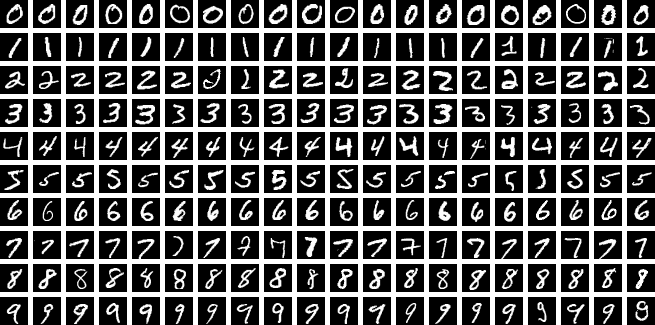
\includegraphics[width=12cm]{mnist.png}
\end{center}

\bigskip

\begin{center}

\includegraphics[width=4cm]{digit.png}
\end{center}

\bigskip

{\tiny
\begin{verbatim}
[[  0   0   0   0   0   0   0   0   0   0   0   0   0   0   0   0   0   0   0   0   0   0   0   0   0   0   0   0]
 [  0   0   0   0   0   0   0   0   0   0   0   0   0   0   0   0   0   0   0   0   0   0   0   0   0   0   0   0]
 [  0   0   0   0   0   0   0   0   0   0   0   0   0   0   0   0   0   0   0   0   0   0   0   0   0   0   0   0]
 [  0   0   0   0   0   0   0   0   0   0   0   0   0   0   0   0   0   0   0   0   0   0   0   0   0   0   0   0]
 [  0   0   0   0   0   0   0   0   0   0   0   0   0   0   0   0   0   0   0   0   0   0   0   0   0   0   0   0]
 [  0   0   0   0   0   0   0   0   0   0   0   0   0   0   0   0   0   0   0   0   0   0   0   0   0   0   0   0]
 [  0   0   0   0   0   0   0   0   0   0   0   0   0   0   0   0   0   0   0   0   0   0   0   0   0   0   0   0]
 [  0   0   0   0   0   0  84 185 159 151  60  36   0   0   0   0   0   0   0   0   0   0   0   0   0   0   0   0]
 [  0   0   0   0   0   0 222 254 254 254 254 241 198 198 198 198 198 198 198 198 170  52   0   0   0   0   0   0]
 [  0   0   0   0   0   0  67 114  72 114 163 227 254 225 254 254 254 250 229 254 254 140   0   0   0   0   0   0]
 [  0   0   0   0   0   0   0   0   0   0   0  17  66  14  67  67  67  59  21 236 254 106   0   0   0   0   0   0]
 [  0   0   0   0   0   0   0   0   0   0   0   0   0   0   0   0   0   0  83 253 209  18   0   0   0   0   0   0]
 [  0   0   0   0   0   0   0   0   0   0   0   0   0   0   0   0   0  22 233 255  83   0   0   0   0   0   0   0]
 [  0   0   0   0   0   0   0   0   0   0   0   0   0   0   0   0   0 129 254 238  44   0   0   0   0   0   0   0]
 [  0   0   0   0   0   0   0   0   0   0   0   0   0   0   0   0  59 249 254  62   0   0   0   0   0   0   0   0]
 [  0   0   0   0   0   0   0   0   0   0   0   0   0   0   0   0 133 254 187   5   0   0   0   0   0   0   0   0]
 [  0   0   0   0   0   0   0   0   0   0   0   0   0   0   0   9 205 248  58   0   0   0   0   0   0   0   0   0]
 [  0   0   0   0   0   0   0   0   0   0   0   0   0   0   0 126 254 182   0   0   0   0   0   0   0   0   0   0]
 [  0   0   0   0   0   0   0   0   0   0   0   0   0   0  75 251 240  57   0   0   0   0   0   0   0   0   0   0]
 [  0   0   0   0   0   0   0   0   0   0   0   0   0  19 221 254 166   0   0   0   0   0   0   0   0   0   0   0]
 [  0   0   0   0   0   0   0   0   0   0   0   0   3 203 254 219  35   0   0   0   0   0   0   0   0   0   0   0]
 [  0   0   0   0   0   0   0   0   0   0   0   0  38 254 254  77   0   0   0   0   0   0   0   0   0   0   0   0]
 [  0   0   0   0   0   0   0   0   0   0   0  31 224 254 115   1   0   0   0   0   0   0   0   0   0   0   0   0]
 [  0   0   0   0   0   0   0   0   0   0   0 133 254 254  52   0   0   0   0   0   0   0   0   0   0   0   0   0]
 [  0   0   0   0   0   0   0   0   0   0  61 242 254 254  52   0   0   0   0   0   0   0   0   0   0   0   0   0]
 [  0   0   0   0   0   0   0   0   0   0 121 254 254 219  40   0   0   0   0   0   0   0   0   0   0   0   0   0]
 [  0   0   0   0   0   0   0   0   0   0 121 254 207  18   0   0   0   0   0   0   0   0   0   0   0   0   0   0]
 [  0   0   0   0   0   0   0   0   0   0   0   0   0   0   0   0   0   0   0   0   0   0   0   0   0   0   0   0]]
\end{verbatim}
}

\clearpage

\SectionTitle{Neural Network}

\begin{center}
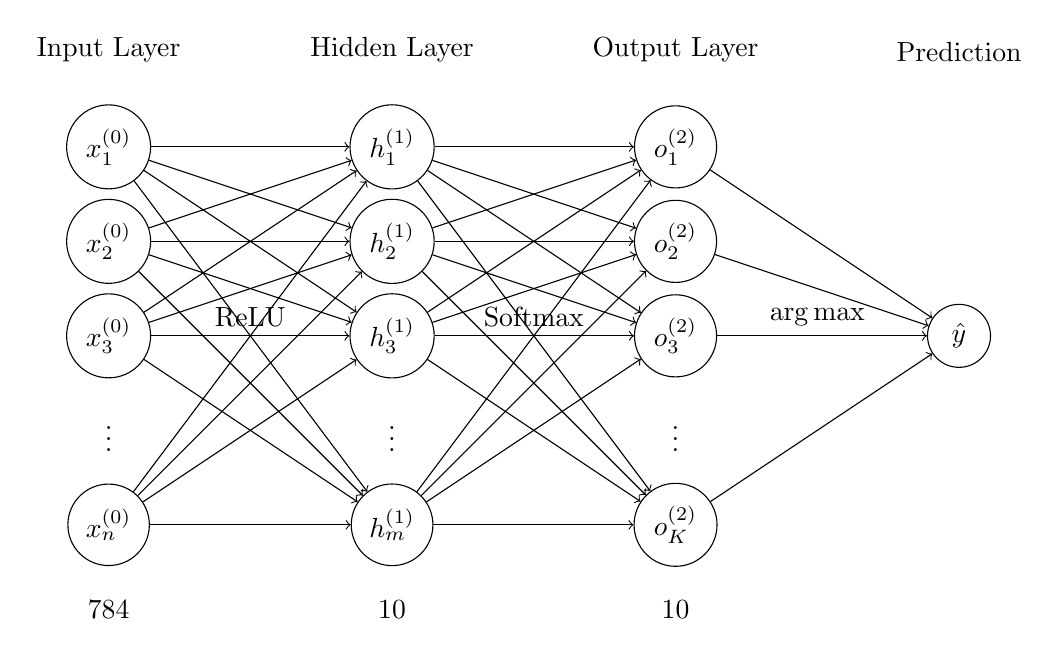
\begin{tikzpicture}[
  x=1.8cm, y=1.2cm,
  neuron/.style={circle, draw, minimum size=8mm},
  dots/.style={draw=none, minimum size=4mm}
]

\node[above] at (0, 1.8) {Input Layer};
\node[above] at (2, 1.8) {Hidden Layer};
\node[above] at (4, 1.8) {Output Layer};
\node[above] at (6, 1.8) {Prediction};

\node[below] at (0, -3.7) {784};
\node[below] at (2, -3.7) {10};
\node[below] at (4, -3.7) {10};

\node[neuron] (I1) at (0, 1) {$x_1^{(0)}$};
\node[neuron] (I2) at (0, 0) {$x_2^{(0)}$};
\node[neuron] (I3) at (0, -1) {$x_3^{(0)}$};
\node[dots] (Idots) at (0, -2) {$\vdots$};
\node[neuron] (In) at (0, -3) {$x_n^{(0)}$};

\node[neuron] (H1) at (2, 1) {$h_1^{(1)}$};
\node[neuron] (H2) at (2, 0) {$h_2^{(1)}$};
\node[neuron] (H3) at (2, -1) {$h_3^{(1)}$};
\node[dots] (Hdots) at (2, -2) {$\vdots$};
\node[neuron] (Hm) at (2, -3) {$h_m^{(1)}$};

\node[neuron] (H21) at (4, 1) {$o_1^{(2)}$};
\node[neuron] (H22) at (4, 0) {$o_2^{(2)}$};
\node[neuron] (H23) at (4, -1) {$o_3^{(2)}$};
\node[dots] (H2dots) at (4, -2) {$\vdots$};
\node[neuron] (H2m) at (4, -3) {$o_K^{(2)}$};

\node[neuron] (O) at (6, -1) {$\hat{y}$};

\node[above, rotate=0] at (1, -1) {ReLU};
\node[above, rotate=0] at (3, -1) {Softmax};
\node[above, rotate=0] at (5, -1) {$\argmax$};

\foreach \i in {I1,I2,I3,In} {
  \foreach \j in {H1,H2,H3,Hm} {
    \draw[->] (\i) -- (\j);
  }
}

\foreach \i in {H1,H2,H3,Hm} {
  \foreach \j in {H21,H22,H23,H2m} {
    \draw[->] (\i) -- (\j);
  }
}

\foreach \i in {H21,H22,H23,H2m} {
  \draw[->] (\i) -- (O);
}

\end{tikzpicture}
\end{center}

\bigskip

\begin{itemize}
  \item \textbf{Neuron} - Basic computational unit that processes inputs
  \item \textbf{Weight ($w$)} - Connection strength between neurons
  \item \textbf{Bias ($b$)} - Offset value added to weighted sum
  \item \textbf{Forward propagation} - Computing outputs from inputs through the network
  \item \textbf{Logits ($z$)} - Pre-activation output
  \item \textbf{Activation ($a$)} - Non-linear function applied to neuron outputs
  \item \textbf{Backward propagation} - Computing gradients from outputs back to inputs
  \item \textbf{One-hot} - Binary vector representation of categorical labels
  \item \textbf{Loss ($l$)} - Measure of prediction error to be minimized
  \item \textbf{Gradient ($d$)} - Derivative of loss with respect to a parameter
  \item \textbf{Cross-entropy} - Loss function that measures prediction accuracy
  \item \textbf{Gradient descent} - Optimization algorithm that updates weights and biases
  \item \textbf{Learning rate ($\alpha$)} - Step size for parameter updates in gradient descent
\end{itemize}

\bigskip

\begin{enumerate}
  \item Forward propagation produces predictions
  \item Loss measures how wrong we are
  \item Backward propagation computes gradients from the loss
  \item Gradient descent uses those gradients to update parameters
\end{enumerate}

\clearpage

\SectionTitle{Data Structure}

\[
X =
\begin{bmatrix}
\cdots & x^{(1)} & \cdots \\
\cdots & x^{(2)} & \cdots \\
\vdots & \vdots & \vdots \\
\cdots & x^{(m)} & \cdots
\end{bmatrix}^{\top}
=
\begin{bmatrix}
x^{(1)}_1 & x^{(2)}_1 & \cdots & x^{(m)}_1 \\
x^{(1)}_2 & x^{(2)}_2 & \cdots & x^{(m)}_2 \\
\vdots & \vdots & \ddots & \vdots \\
x^{(1)}_n & x^{(2)}_n & \cdots & x^{(m)}_n
\end{bmatrix}
\]

\clearpage

\SectionTitle{Matrix Multiplication}

\[
C_{ij} = \sum_{p=1}^{k} A_{ip} \cdot B_{pj}
\]

\[
\begin{bmatrix}
0.1 & 0.2 & 0.3 \\
0.4 & 0.5 & 0.6
\end{bmatrix}
\begin{bmatrix}
1 \\
2 \\
3
\end{bmatrix}
=
\begin{bmatrix}
(0.1 \times 1) + (0.2 \times 2) + (0.3 \times 3) \\
(0.4 \times 1) + (0.5 \times 2) + (0.6 \times 3)
\end{bmatrix}
=
\begin{bmatrix}
1.4 \\
3.2
\end{bmatrix}
\]

\clearpage

\SectionTitle{Linear Equation}

\[
y = ax + b
\]

\bigskip

\begin{center}
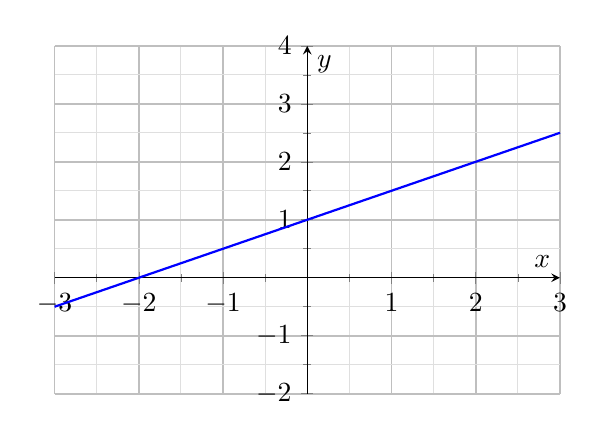
\begin{tikzpicture}
  \begin{axis}[linearplot]
  \addplot[blue, thick] {0.5*x + 1};
  \end{axis}
\end{tikzpicture}
\end{center}

\clearpage

\SectionTitle{ReLU}

\[
\relu(x) = \max(0, x)
\]

\bigskip

\begin{center}
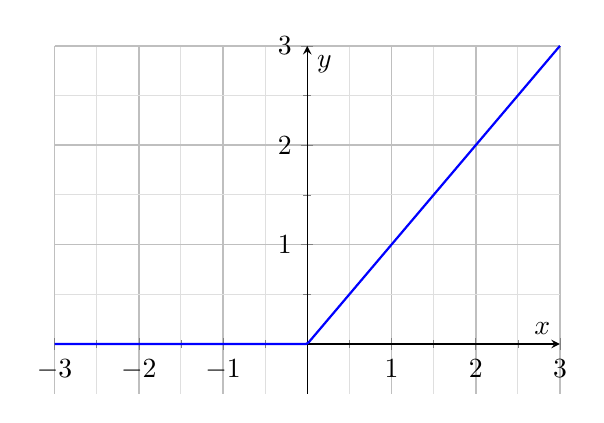
\begin{tikzpicture}
  \begin{axis}[reluplot]
  \addplot[blue, thick] {(x>0)*x};
  \end{axis}
\end{tikzpicture}
\end{center}

\clearpage

\SectionTitle{Softmax}

\[
\softmax(z_i) = \frac{e^{z_i}}{\sum_{j=1}^{K} e^{z_j}} \quad \text{for } i=1,\dots,K.
\]

\bigskip

\begin{center}
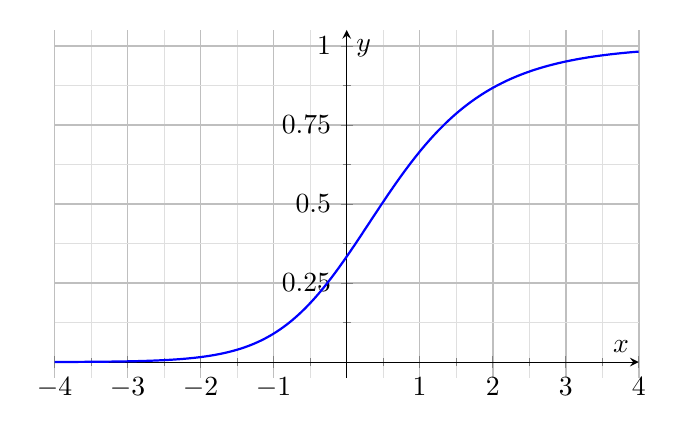
\begin{tikzpicture}
  \begin{axis}[softmaxplot]
  \addplot[blue, thick] {exp(x)/(exp(x)+1+exp(-x))};
  \end{axis}
\end{tikzpicture}
\end{center}

\clearpage

\SectionTitle{Derivative}

\[
f(x) = x^2
\]

\bigskip

\begin{center}
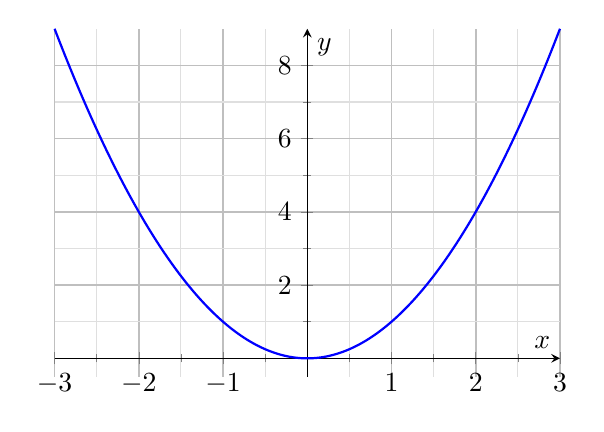
\begin{tikzpicture}
  \begin{axis}[quadraticplot]
  \addplot[blue, thick] {x^2};
  \end{axis}
\end{tikzpicture}
\end{center}

\bigskip

\[
f'(x) = 2x
\]

\bigskip

\begin{center}
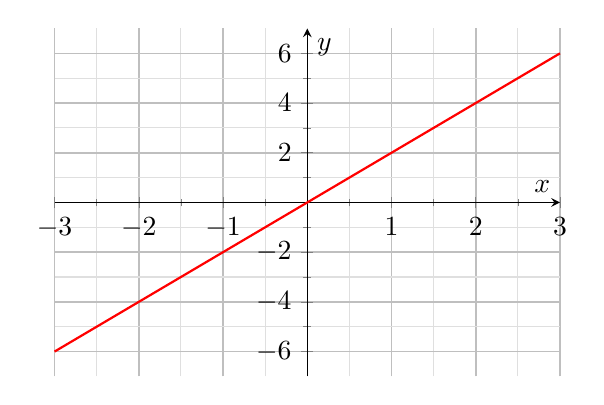
\begin{tikzpicture}
  \begin{axis}[derivativeplot]
  \addplot[red, thick] {2*x};
  \end{axis}
\end{tikzpicture}
\end{center}

\bigskip

The derivative tells us the \textbf{rate of change}: how much the output changes when we make a change to the input.

\clearpage

\SectionTitle{ReLU Derivative}

\[
\relu'(x) = \begin{cases}
0, & x < 0, \\
1, & x > 0, \\
\text{undefined}, & x = 0
\end{cases}
\]

\bigskip

\begin{center}
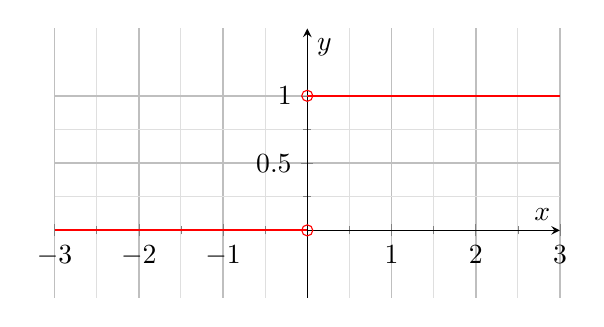
\begin{tikzpicture}
  \begin{axis}[reluderivplot]
  \addplot[red, thick, domain=-3:0] {0};
  \addplot[red, thick, domain=0:3] {1};
  \addplot[red, mark=o, only marks] coordinates {(0,0) (0,1)};
  \end{axis}
\end{tikzpicture}
\end{center}

\bigskip

\[
\relu'(x) = \begin{cases}
0, & x \leq 0, \\
1, & x > 0
\end{cases}
\]

\bigskip

\begin{center}
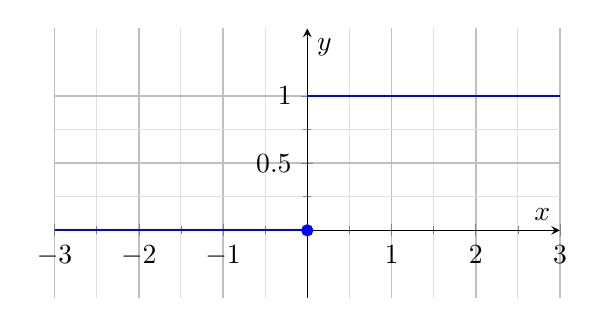
\begin{tikzpicture}
  \begin{axis}[reluderivplot]
  \addplot[blue, thick, domain=-3:0] {0};
  \addplot[blue, thick, domain=0:3] {1};
  \addplot[blue, mark=*, only marks] coordinates {(0,0)};
  \end{axis}
\end{tikzpicture}
\end{center}

\clearpage

\SectionTitle{Cross-Entropy Loss}

\[
L = -\sum_{i=0}^{C-1} y_i \log(\hat{y}_i)
\]

\bigskip

Where:
\begin{itemize}
  \item $C$ = number of classes
  \item $y_i$ = true label (one-hot encoded): 1 if class $i$ is correct, 0 otherwise
  \item $\hat{y}_i$ = predicted probability for class $i$ (output from softmax)
\end{itemize}

\bigskip

\textbf{Key Properties:}
\begin{itemize}
  \item If prediction is perfect ($\hat{y} = 1$ for correct class): $L = -\log(1) = 0$
  \item If prediction is terrible ($\hat{y} \to 0$ for correct class): $L \to \infty$
  \item Only the correct class contributes to the loss (all other $y_i = 0$)
\end{itemize}

\bigskip

\begin{center}
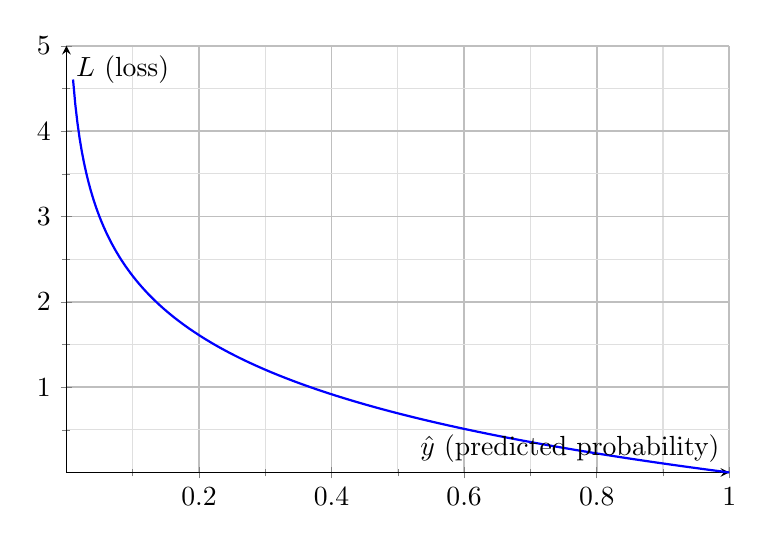
\begin{tikzpicture}
  \begin{axis}[crossentropyplot]
  \addplot[blue, thick] {-ln(x)};
  \end{axis}
\end{tikzpicture}
\end{center}


\end{document}
